% Copyright 2019 Clara Eleonore Pavillet

% Author: Clara Eleonore Pavillet
% Description: This is an unofficial Oxford University Beamer Template I made from scratch. Feel free to use it, modify it, share it.
% Version: 1.0

\documentclass{beamer}
% Load Packages
\usepackage[utf8]{inputenc}
\usepackage{xcolor}
\usepackage{tikz}
\usetikzlibrary{positioning,calc}
\usepackage{graphicx}
\usepackage{hyperref}
\usepackage{amsmath}
\usepackage{listings}
%\usepackage{fontawesome}

% Define Commands
\newcommand*{\ClipSep}{0.06cm} %To adjust footer logo
\newcommand{\E}{\mathrm{e}\,} %\def\I{e} % used to defined e for exp(x), see later what it should be
\newcommand{\ud}{\mathrm{d}}
\lstset{numbers=left, numberstyle=\tiny, stepnumber=1,firstnumber=1,breaklines=true,
    numbersep=5pt,language=Python,
    stringstyle=\ttfamily,
    basicstyle=\footnotesize, 
    showstringspaces=false
}

\usetheme{oxonian}

\title{LXe scintillation model}
\begin{document}

{\setbeamertemplate{footline}{} 
\frame{\titlepage}}

\begin{frame}{Game plan}
\begin{itemize}
\item Use averaged PMT signals from several data sets to find parameters that best fit models.\\
\item Compare fits of different models to find which model is more likely.
\end{itemize}  
\begin{figure}[H]
  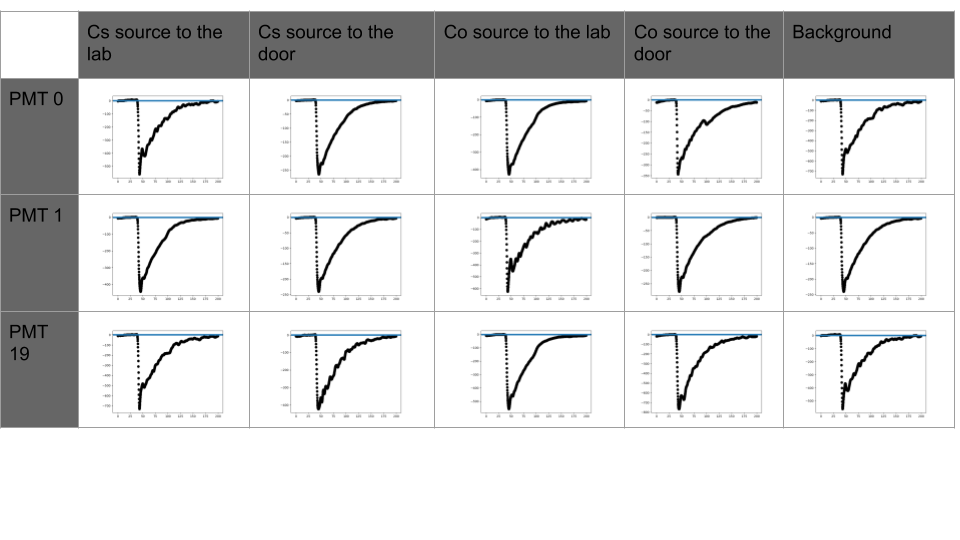
\includegraphics[width=\linewidth]{WFs.png}
  \label{fig:boat1}
\end{figure}
\end{frame}

%\begin{frame}{Averaged signal as model tester}
%\begin{equation}
%    wf_i=\sum_kN_kR^k_i=\sum_k\sum_{n_k=1}^{N_k}spe_{i-k-j}, \quad j\sim Norm(0,\sigma)
%\end{equation}

%\begin{equation}
%\begin{split}
%    WF_i=&\frac{1}{M}\sum_awf_{i-j}^a, \quad j\sim Norm(0,\sigma)\\
%    WF_i=&\frac{1}{M}\sum_{j}\sum_{a_j}wf_{i-j}^{a_j}=\frac{1}{M}\sum_{j,k}\sum_{a_j}\sum_{n=1}^{N_k}spe_{i-j-k-l}\\
%l\sim&Norm(0,\sigma)\\
%WF_i=&\frac{1}{M}\sum_{j,k}\sum_{a_j}N_k\langle spe\rangle_{i-j-k}=\\
%&\frac{1}{\sqrt{2\pi}\sigma}\sum_{j,k}\langle N\rangle_k\langle spe\rangle_{i-j-k}e^{-(j-T_0)^2/2\sigma^2}
%\end{split}
%\end{equation}
%\end{frame}

\begin{frame}{Averaged PMT signal as model tester}
\begin{equation}
\begin{split}
 &WF_{i,a}=\frac{dx}{\sqrt{2\pi}\sigma_a}\left[\langle N_a\rangle*\left(\langle spe_a\rangle*e^{-T_0^2/2\sigma^2_a}\right)\right]\\
&\underbrace{\langle N\rangle_{t=i,PMT=a}}_{\text{\parbox{3cm}{Average number of pes detected by PMT a at time t.}}}=\underbrace{\langle PEs\rangle}_{\text{\parbox{3cm}{Dataset average of photons emitted per event.}}}\overbrace{Q_a}^{\text{LCE}}\underbrace{P(t,\theta_a,\phi_a)}_{\text{Scintillation model}}
\end{split}
\end{equation}
Parameters to fit:
\begin{itemize}
\item Model parameters:...\\
\item Dataset parameters: $\langle PEs\rangle$, $\hat{z}$.
\item PMT parameters: $Q, T_0, \sigma, \theta, \phi.$ 
\end{itemize}
\end{frame}

\begin{frame}{Models to compare}
The standard scintillation model:
\begin{equation}
\begin{split}
    P(t,\theta,\phi)=&P_0(t)=\frac{F}{4\pi\tau_f}e^{-t/\tau_f}+\frac{1-F}{4\pi\tau_s}e^{-t/\tau_s}\\
    0<F&<1, \quad \tau_f\sim5~ns, \quad \tau_s\sim45~ns
\end{split}
\end{equation}

The proposed scintillation model:
\begin{equation}
\begin{split}
    P(t,\theta,\phi)=&R_0R(\theta,\phi)\delta(t)+(1-R_0)P_0(t)\\
    0<R_0&<1, \quad \int R(\theta,\phi)d\Omega=1\\
   R(\theta,\phi)=&\frac{e^{-(cos\theta-1)^2/2\zeta^2}+e^{-(cos\theta+1)^2/2\zeta^2}}{4\pi\sqrt{2}\zeta erf(\sqrt{2}/\zeta)}
\end{split}
\end{equation}
\end{frame}

\begin{frame}{Parameters to fit}
\begin{itemize}
\item Model parameters: $\overbrace{R_0, \zeta, F}^{\text{Maybe energy dependent}}, \tau_f, \tau_s.$
\item Dataset parameters: $\langle PEs\rangle$, $\hat{z}$.
\item PMT parameters: $Q, T_0, \sigma, \theta, \phi.$ 
\end{itemize}
\end{frame}

\begin{frame}{PMT 5}
\begin{figure}
\centering
  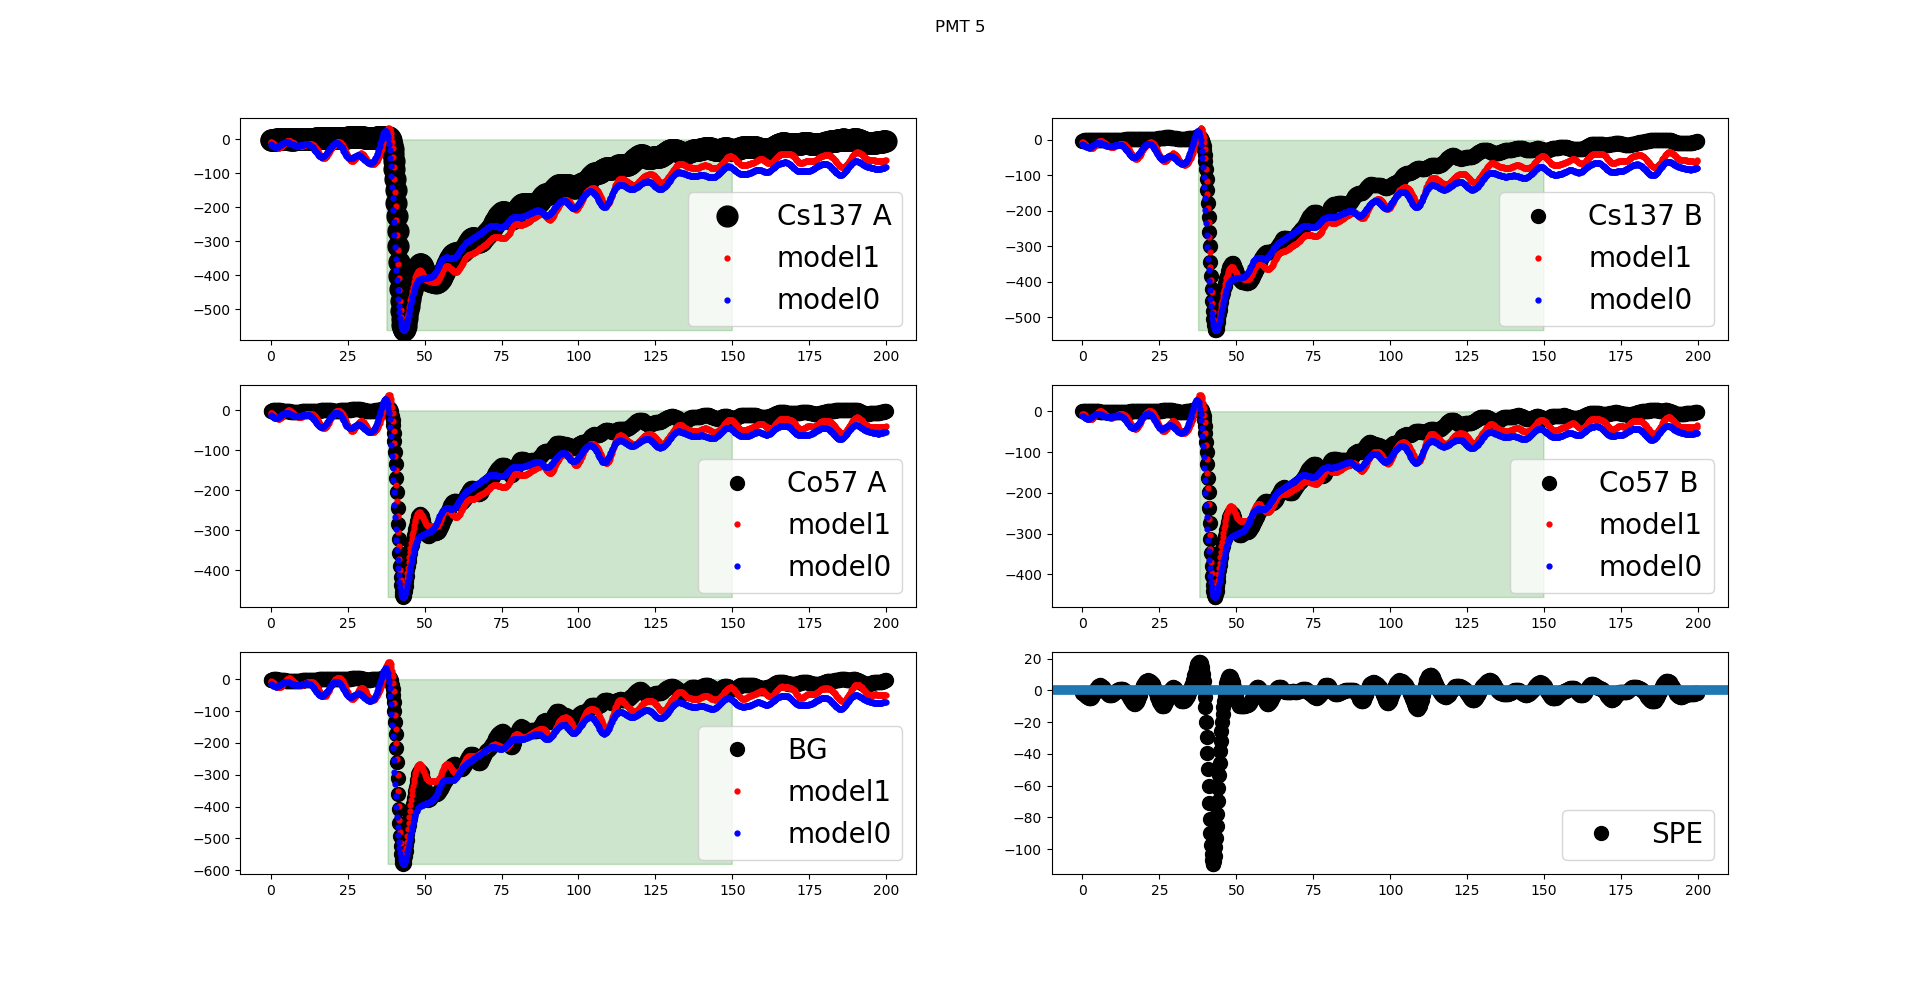
\includegraphics[width=\linewidth]{wf5.png}
\end{figure}
\end{frame}

\begin{frame}{PMT 18}
\begin{figure}[H]
  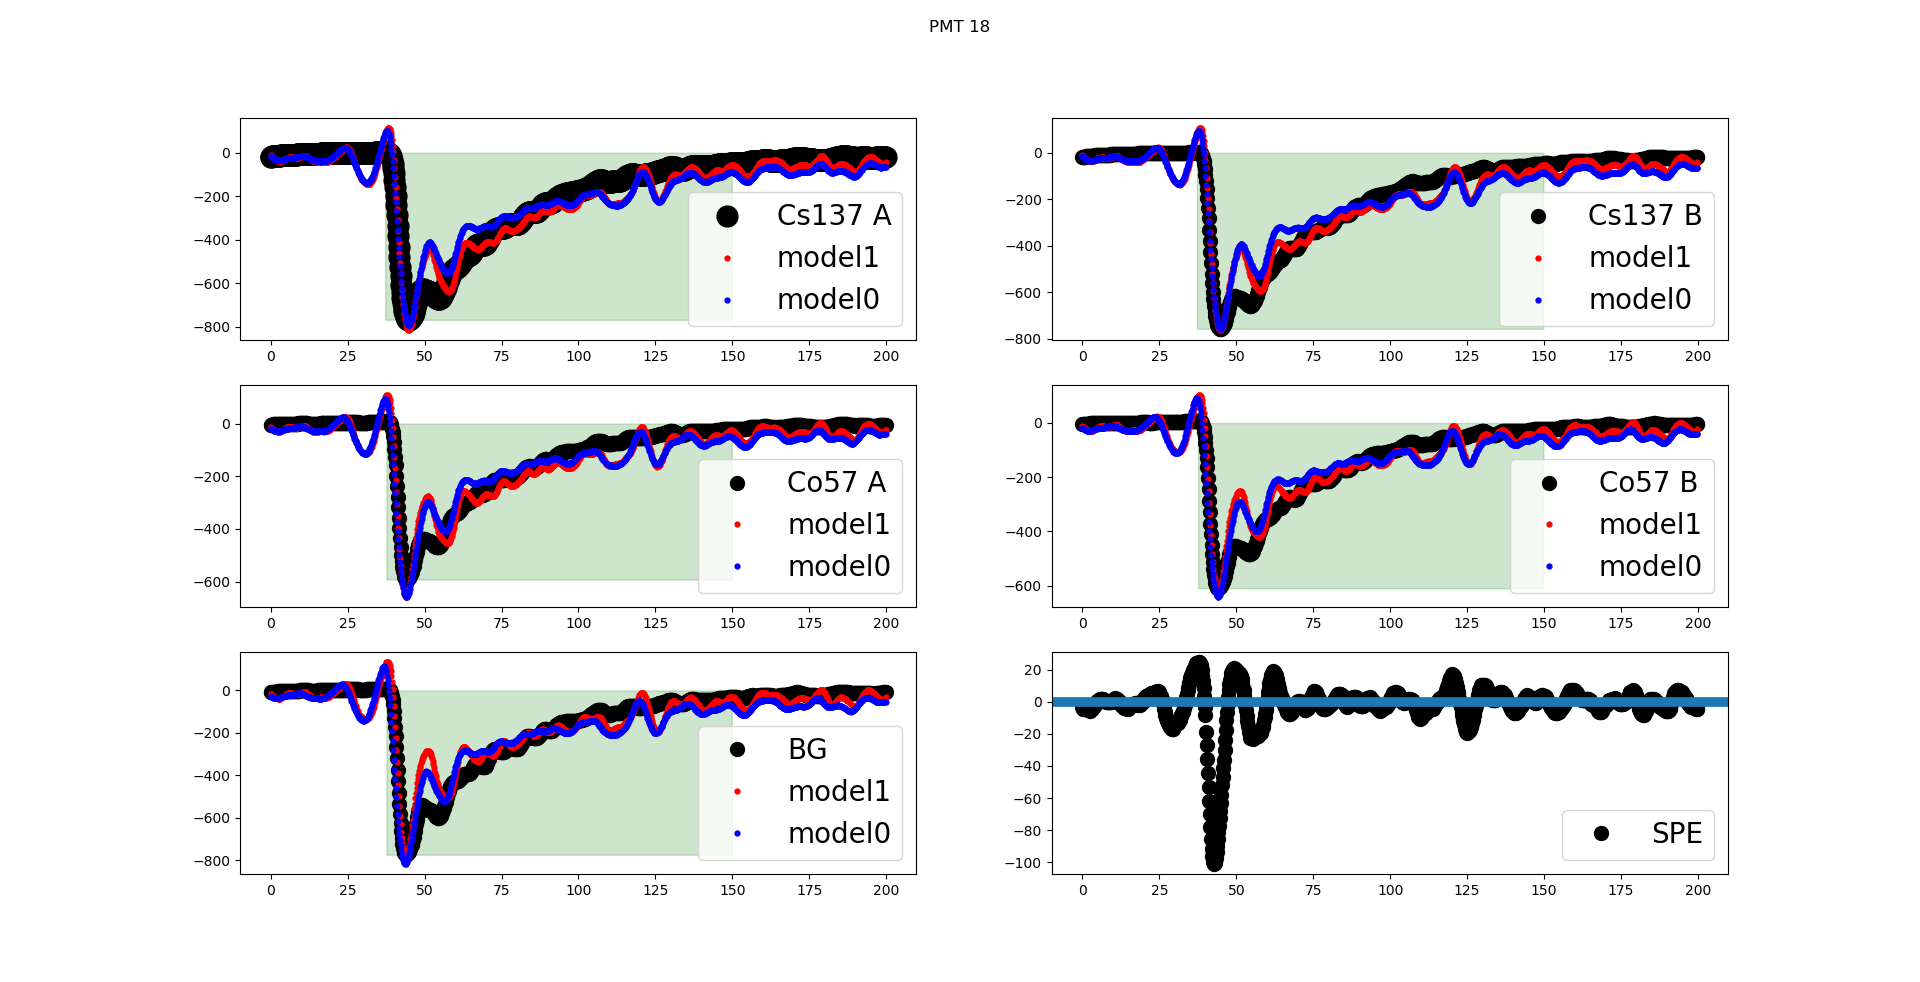
\includegraphics[width=\linewidth]{wf18.png}
\end{figure}
\end{frame}

\begin{frame}{PMT 0}
\begin{figure}[H]
  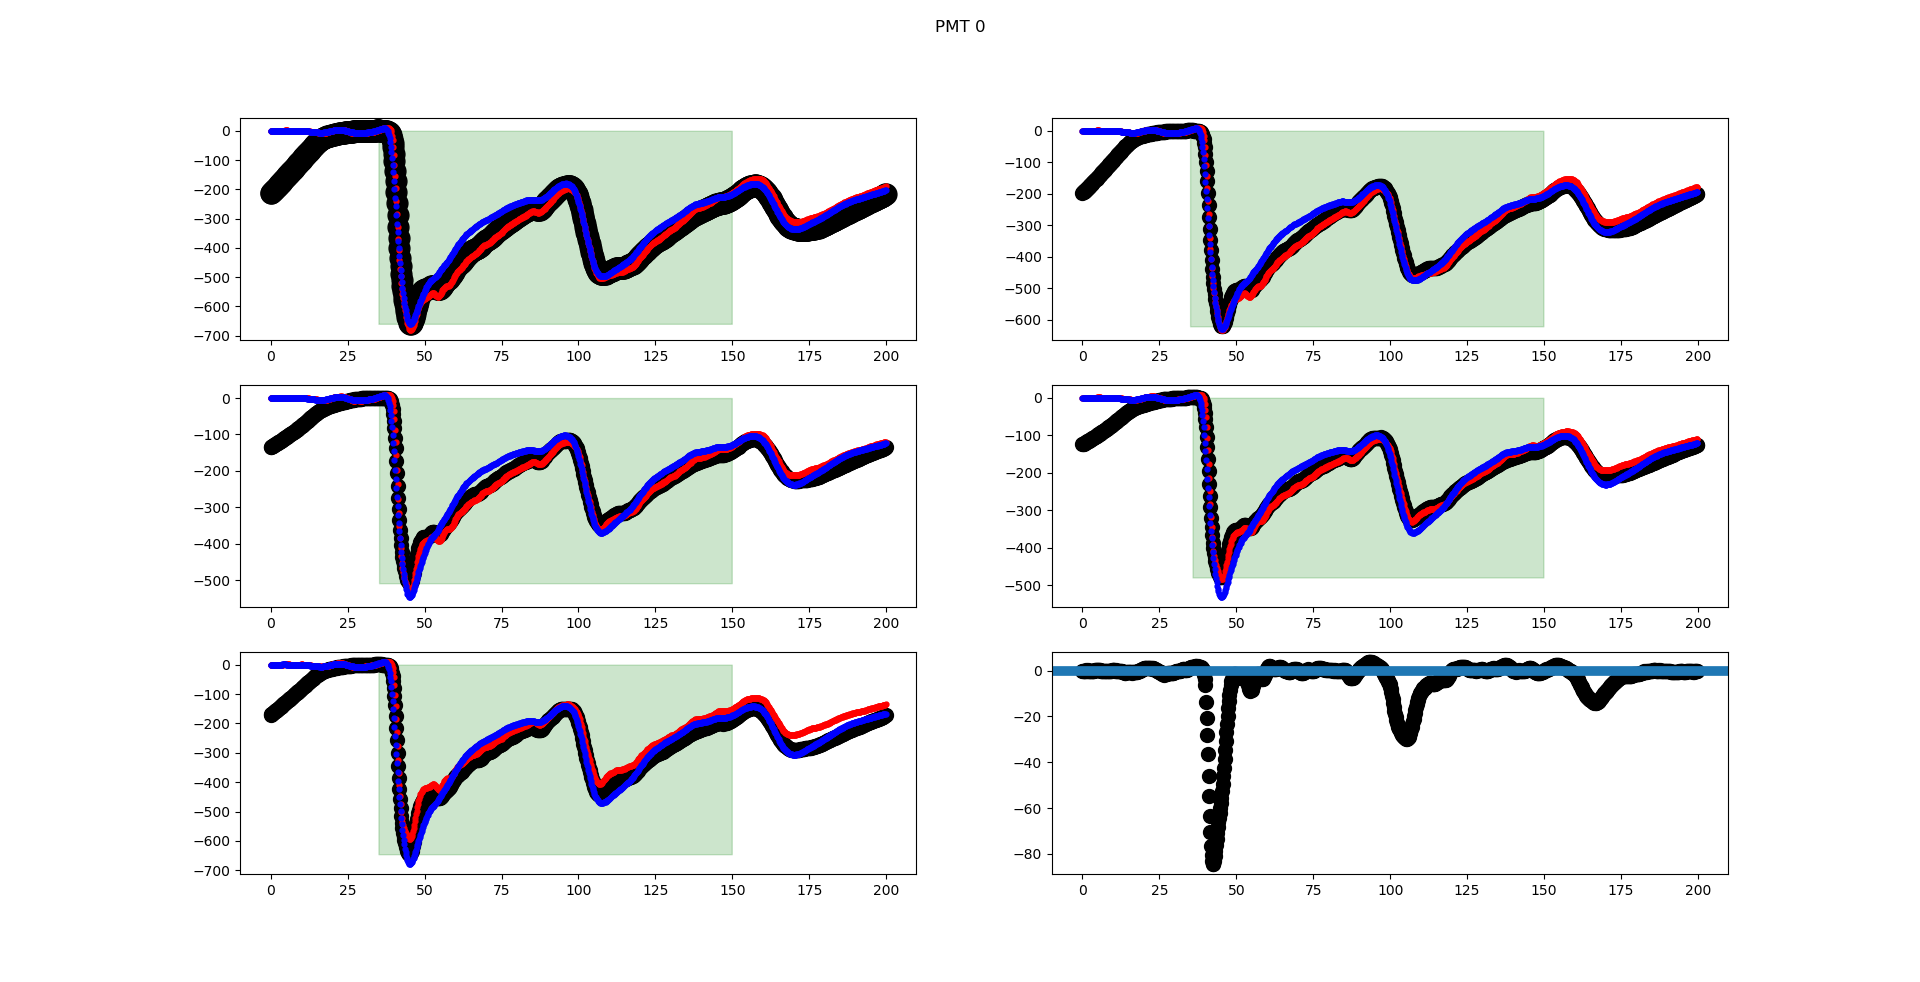
\includegraphics[width=\linewidth]{wf0.png}
\end{figure}
\end{frame}

\begin{frame}{PMT 5}
\begin{figure}[H]
  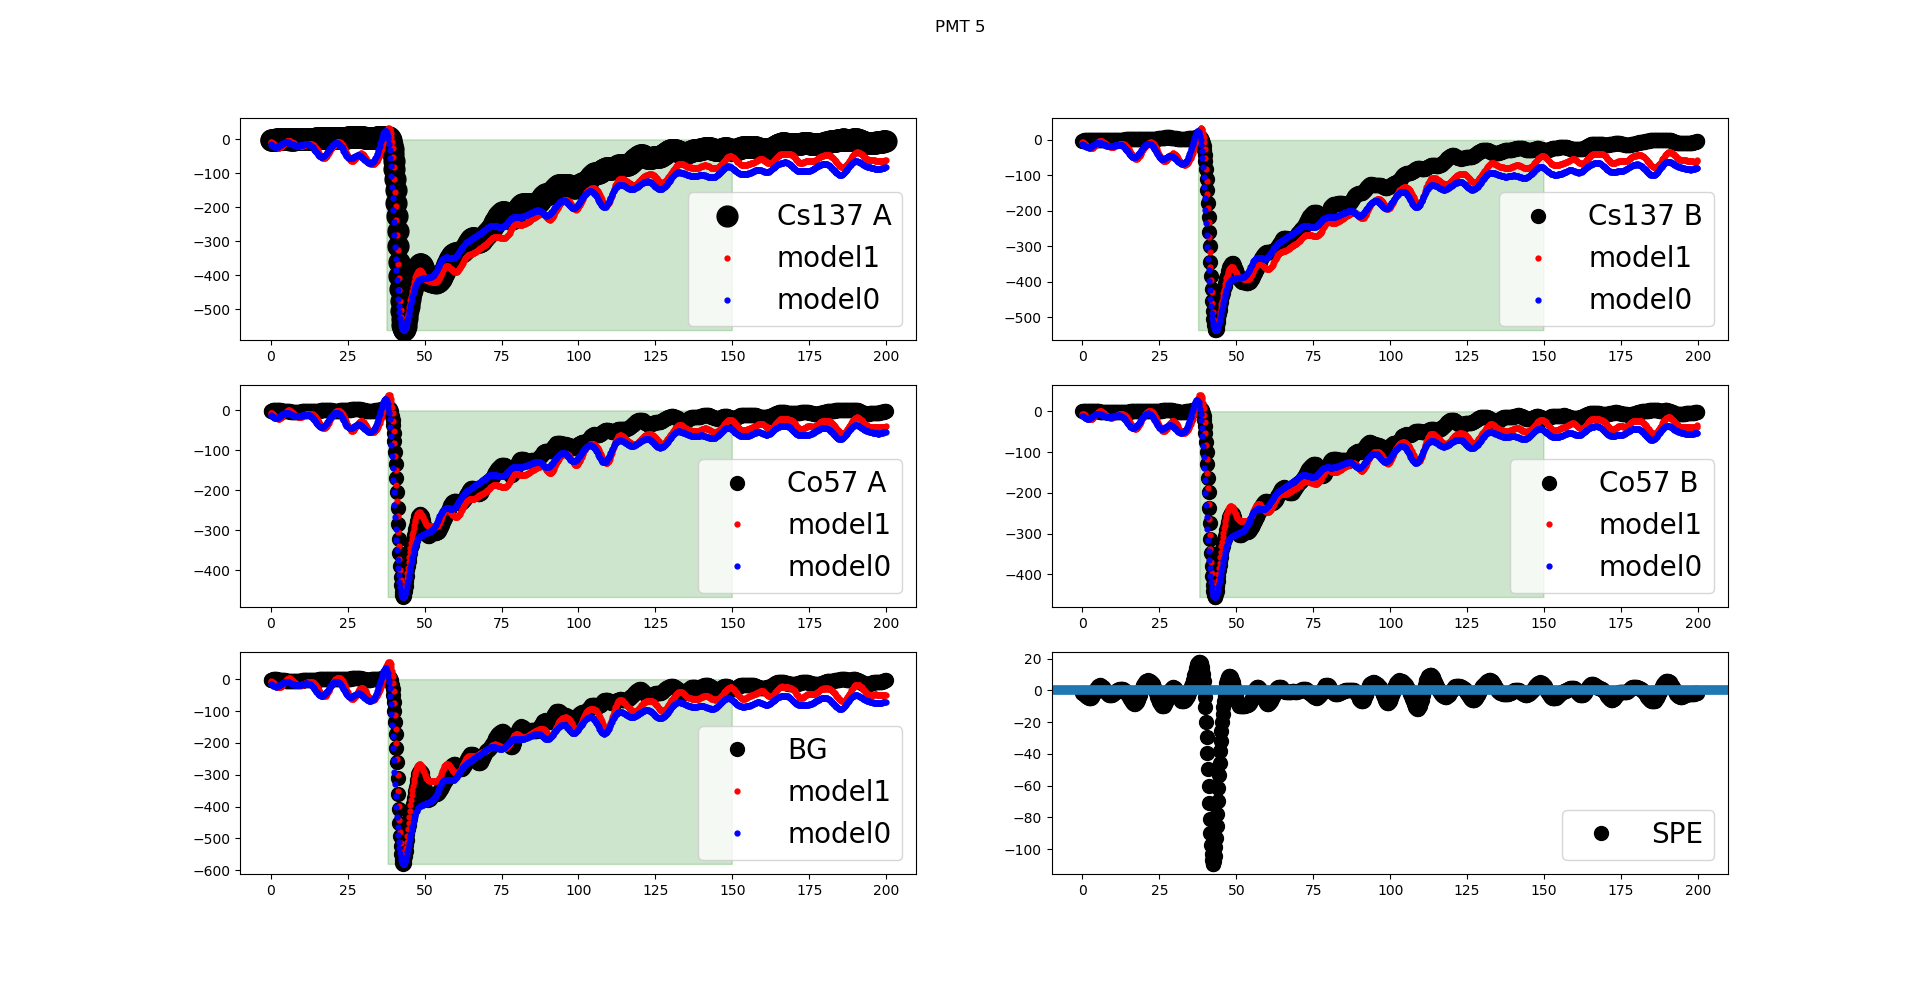
\includegraphics[width=\linewidth]{wf5.png}
\end{figure}
\end{frame}

\begin{frame}{Results - model parameters}

\begin{center}
\begin{tabular}{ |c||c|c| } 
 \hline
 & model 0 & model 1\\ 
 \hline
 \hline
 $\sqrt{\langle\chi^2\rangle}$ & 6.48 &  4.69 \\ 
 \hline
 $\tau_f$~[ns] & 16.38 &  15.5 \\ 
 \hline
  $\tau_s$~[ns] & 69.3 &  58.5 \\ 
 \hline
\end{tabular}
\end{center}
\begin{figure}[h]
  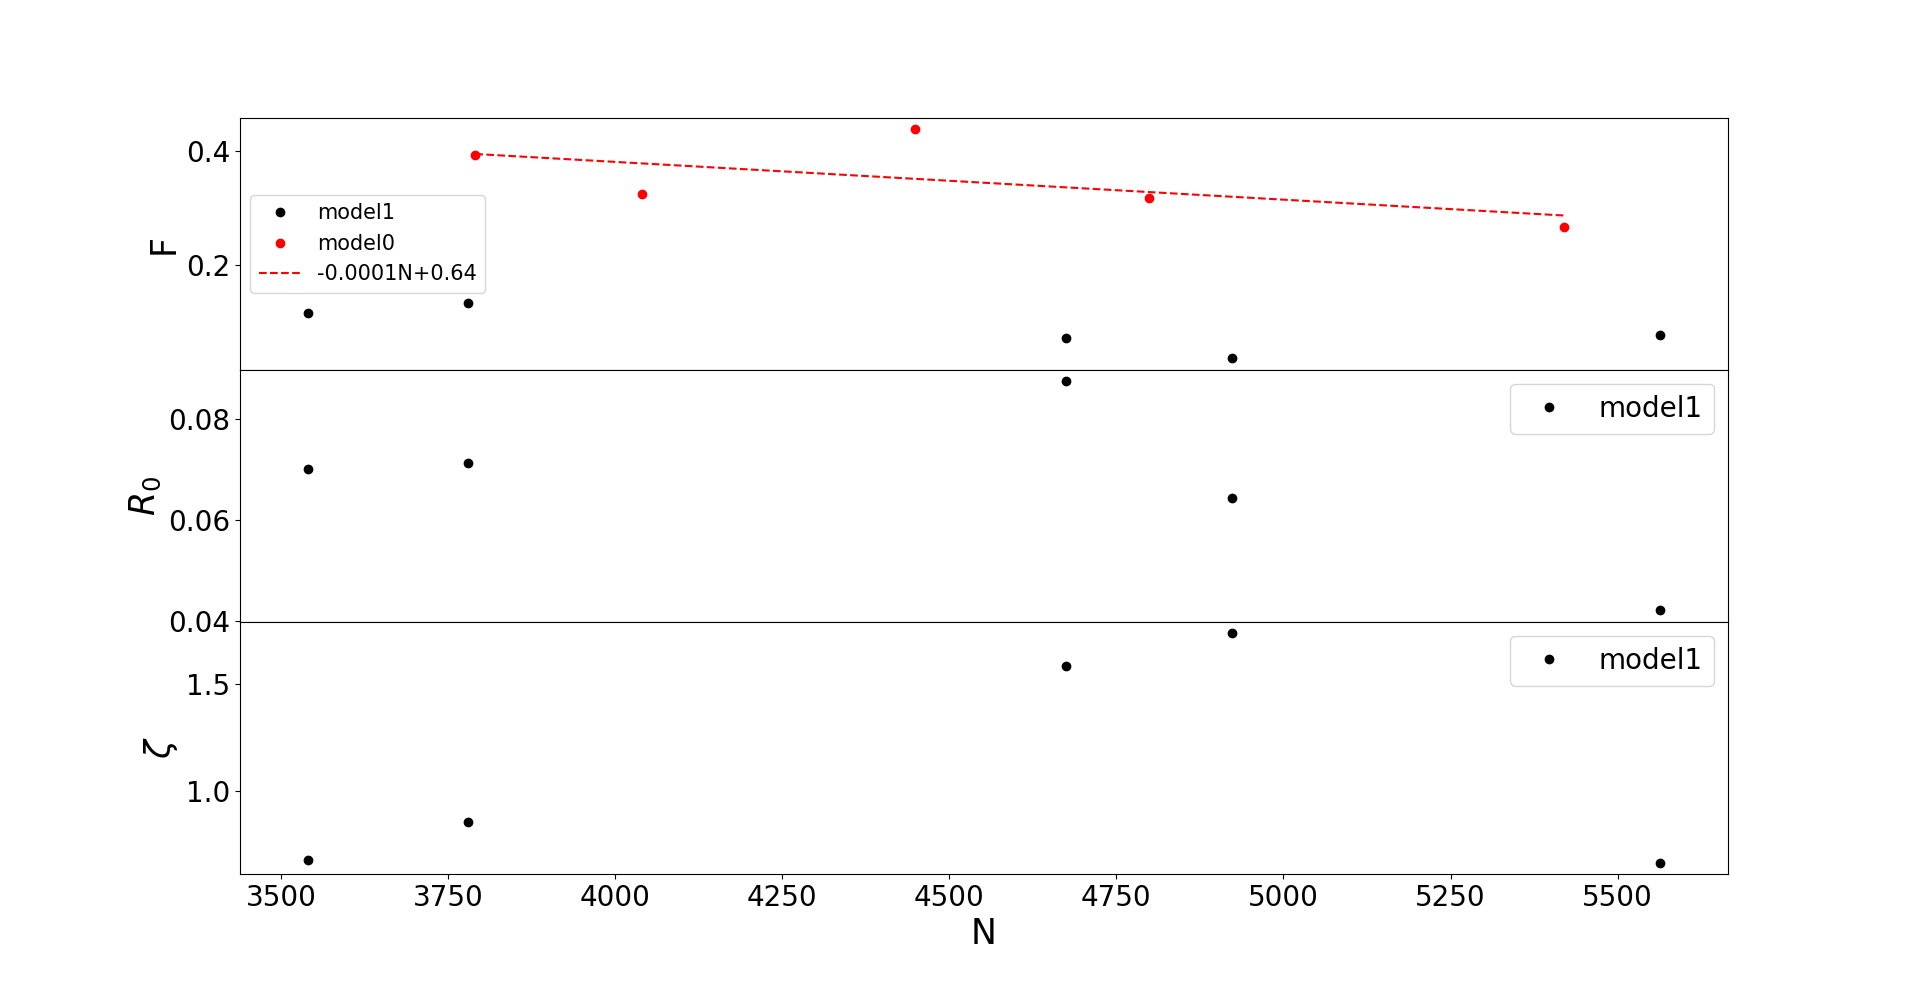
\includegraphics[width=\linewidth]{params.png}
\end{figure}
\tiny{(Model 1 and 0: CoA, CoB, BG, CsB, CsA)}\\
\end{frame}

\begin{frame}{Results - PMT parameters - $\sigma$}
\begin{figure}[h]
  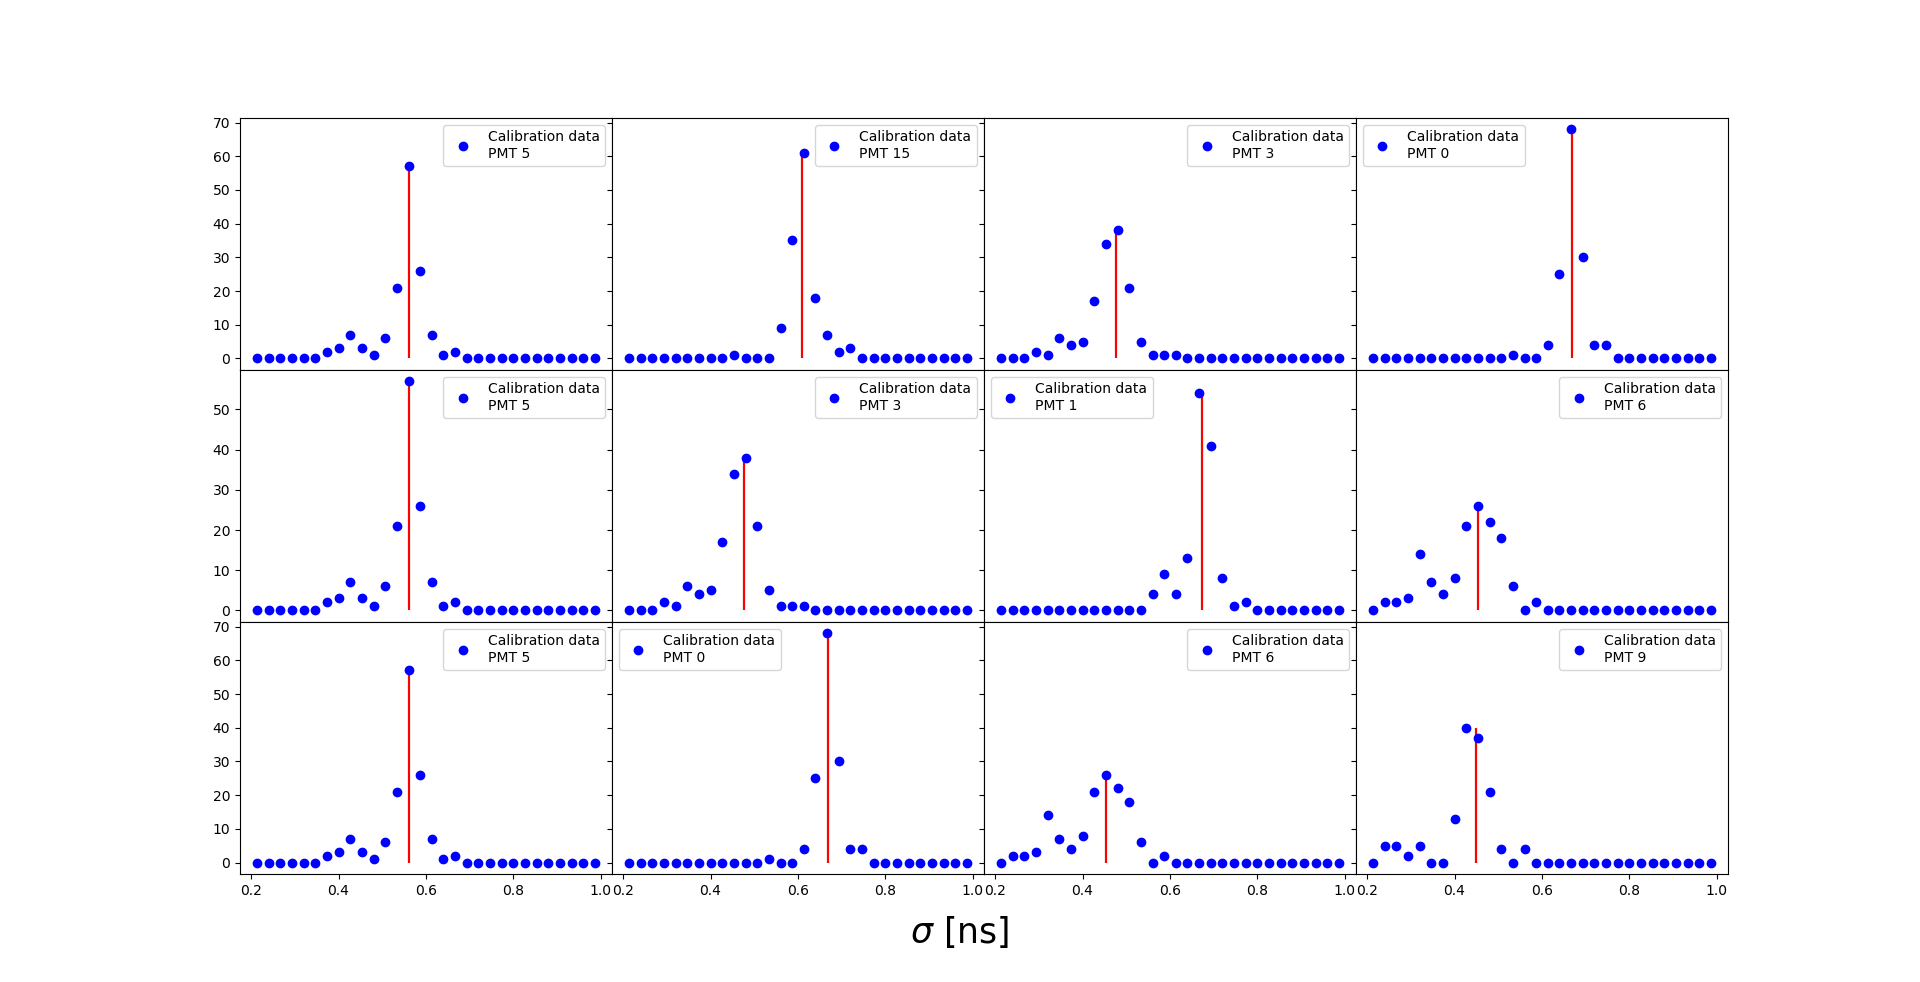
\includegraphics[width=\linewidth]{delay.png}
\end{figure}
\begin{equation}
\sigma_i=0.5\sqrt{\sigma_{ij}^2+\sigma^2_{ik}-\sigma^2_{jk}}
\end{equation}
\end{frame}

\begin{frame}{Results - PMT parameters - Q}
	\begin{figure}[h]
  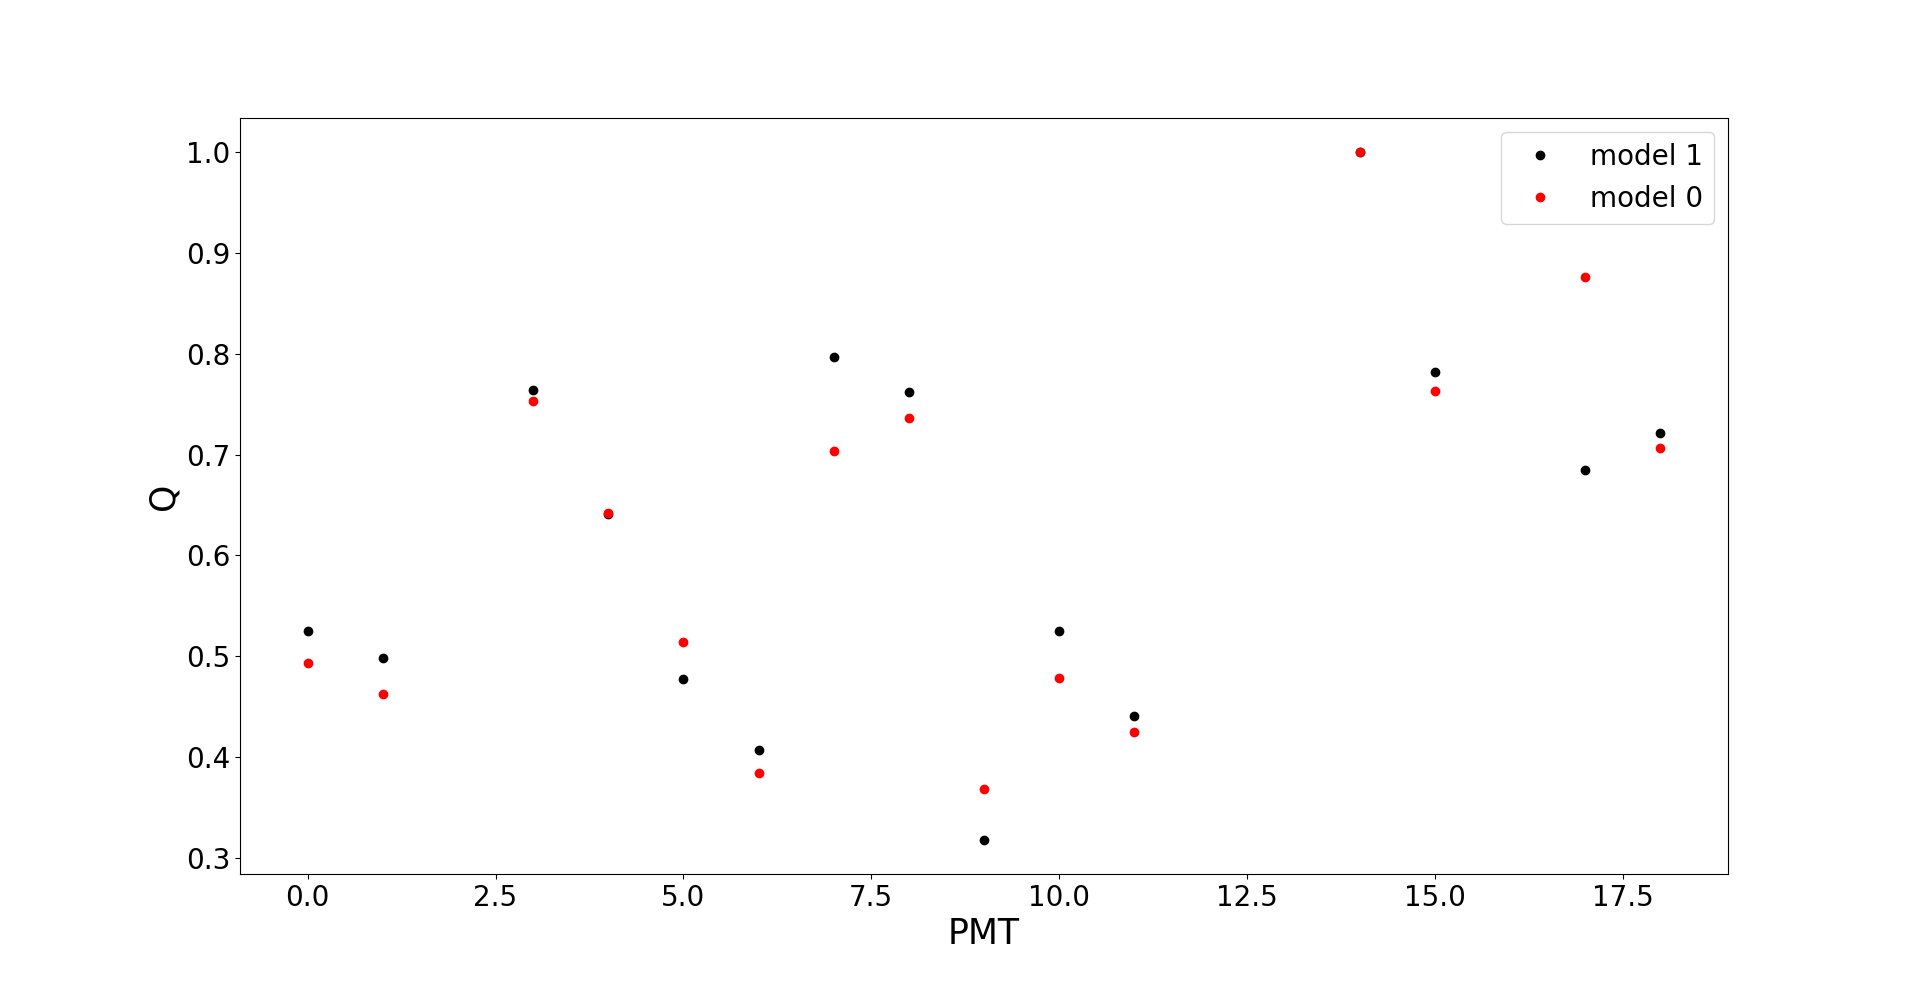
\includegraphics[width=\linewidth]{Q.png}
\end{figure}
\end{frame}

\begin{frame}{Waveform generator}
Create average waveform from a given model:
\begin{itemize}
\item Create N waveforms.
\item Average them with a shift which drawn from Normal$(0,\sigma)$.
\end{itemize}
Create single waveform:
\begin{itemize}
\item Iterate through the 1000 digitized points ($i$) and draw a number of photons to generate $n_i\sim \text{Binom}(\text{Poission}(P_{i,\theta,\phi}), Q)$ 
\item For each generated photon draw an SPE waveform from the calibration data.
\item Add the SPE signal to the waveform at a point $j$ which is drawn from Normal($i,\sigma$).
\end{itemize}
\end{frame}

\begin{frame}{Simulated waveforms}
\begin{figure}[h]
  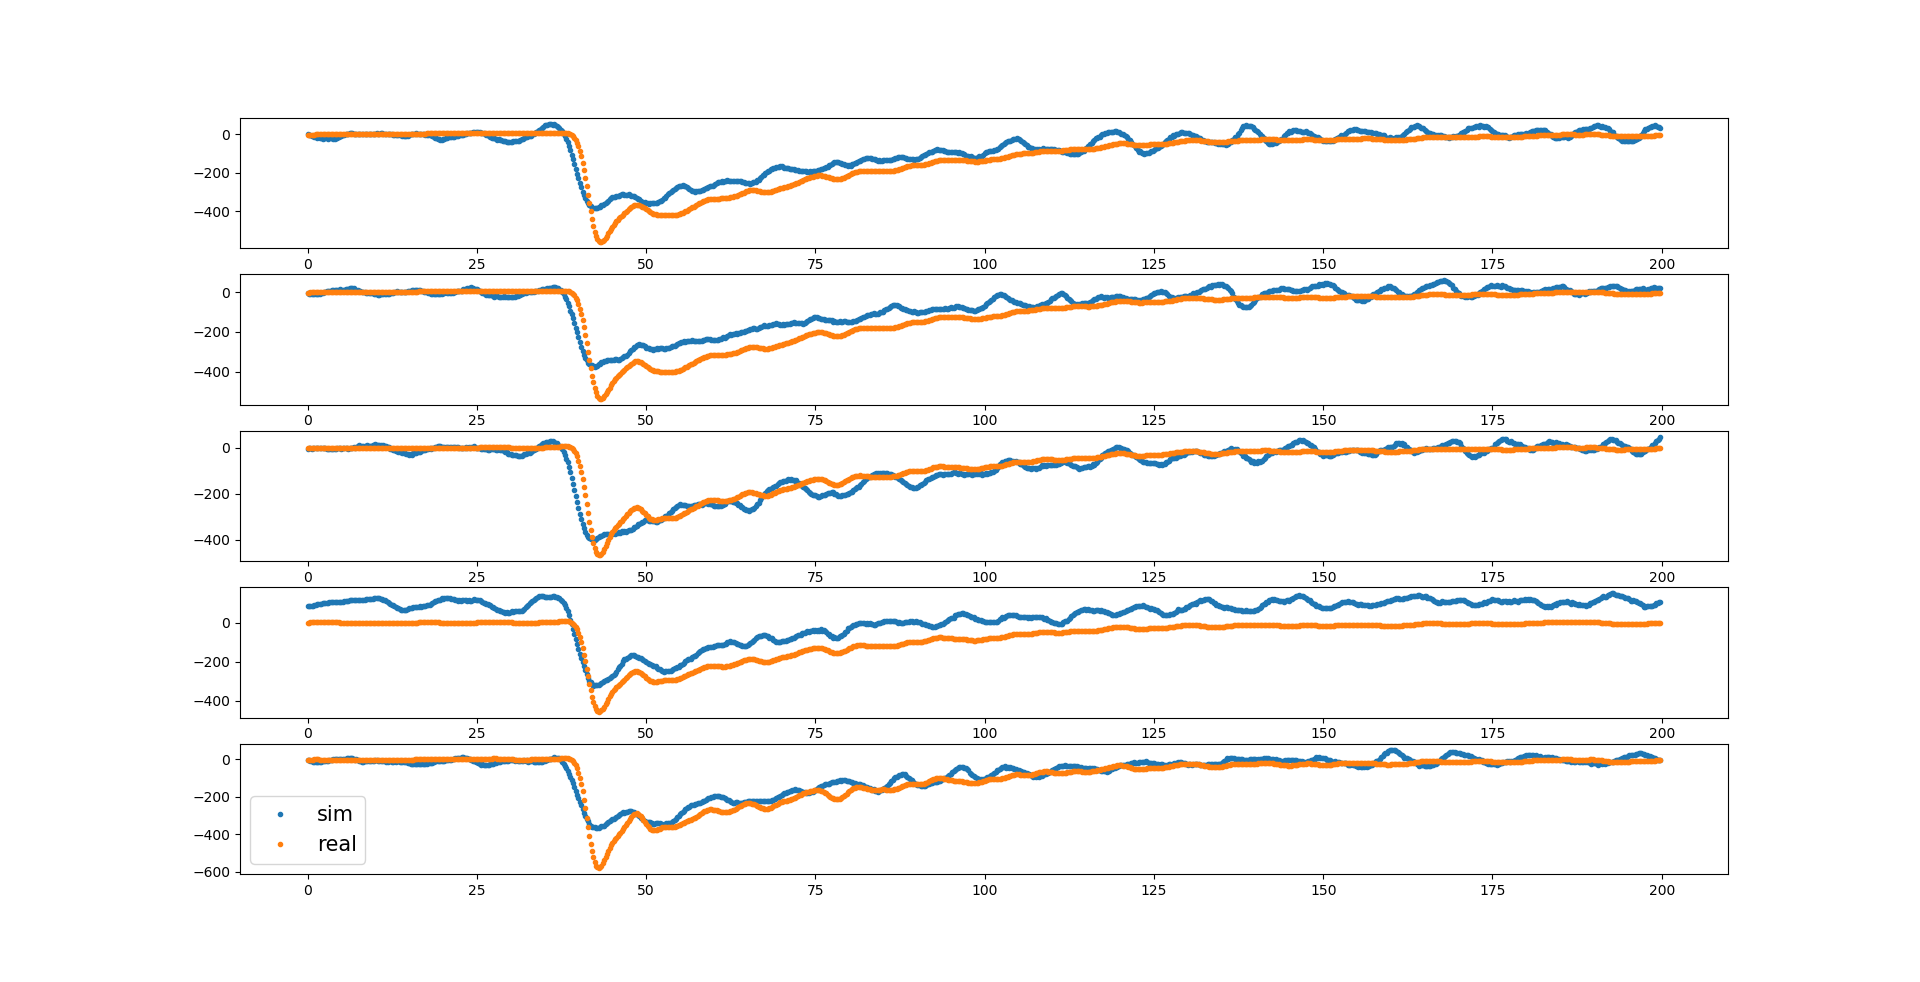
\includegraphics[width=\linewidth]{simWFs.png}
\end{figure}
\end{frame}

\begin{frame}{Significance}
\begin{itemize}
\item Generate datasets with the parameters that best fit model-0 in the real data.
\item Fit it to model-0 and model-1.
\item Compute $\mu=\chi^2_0/\chi^2_1$.
\end{itemize}
\begin{figure}[h]
  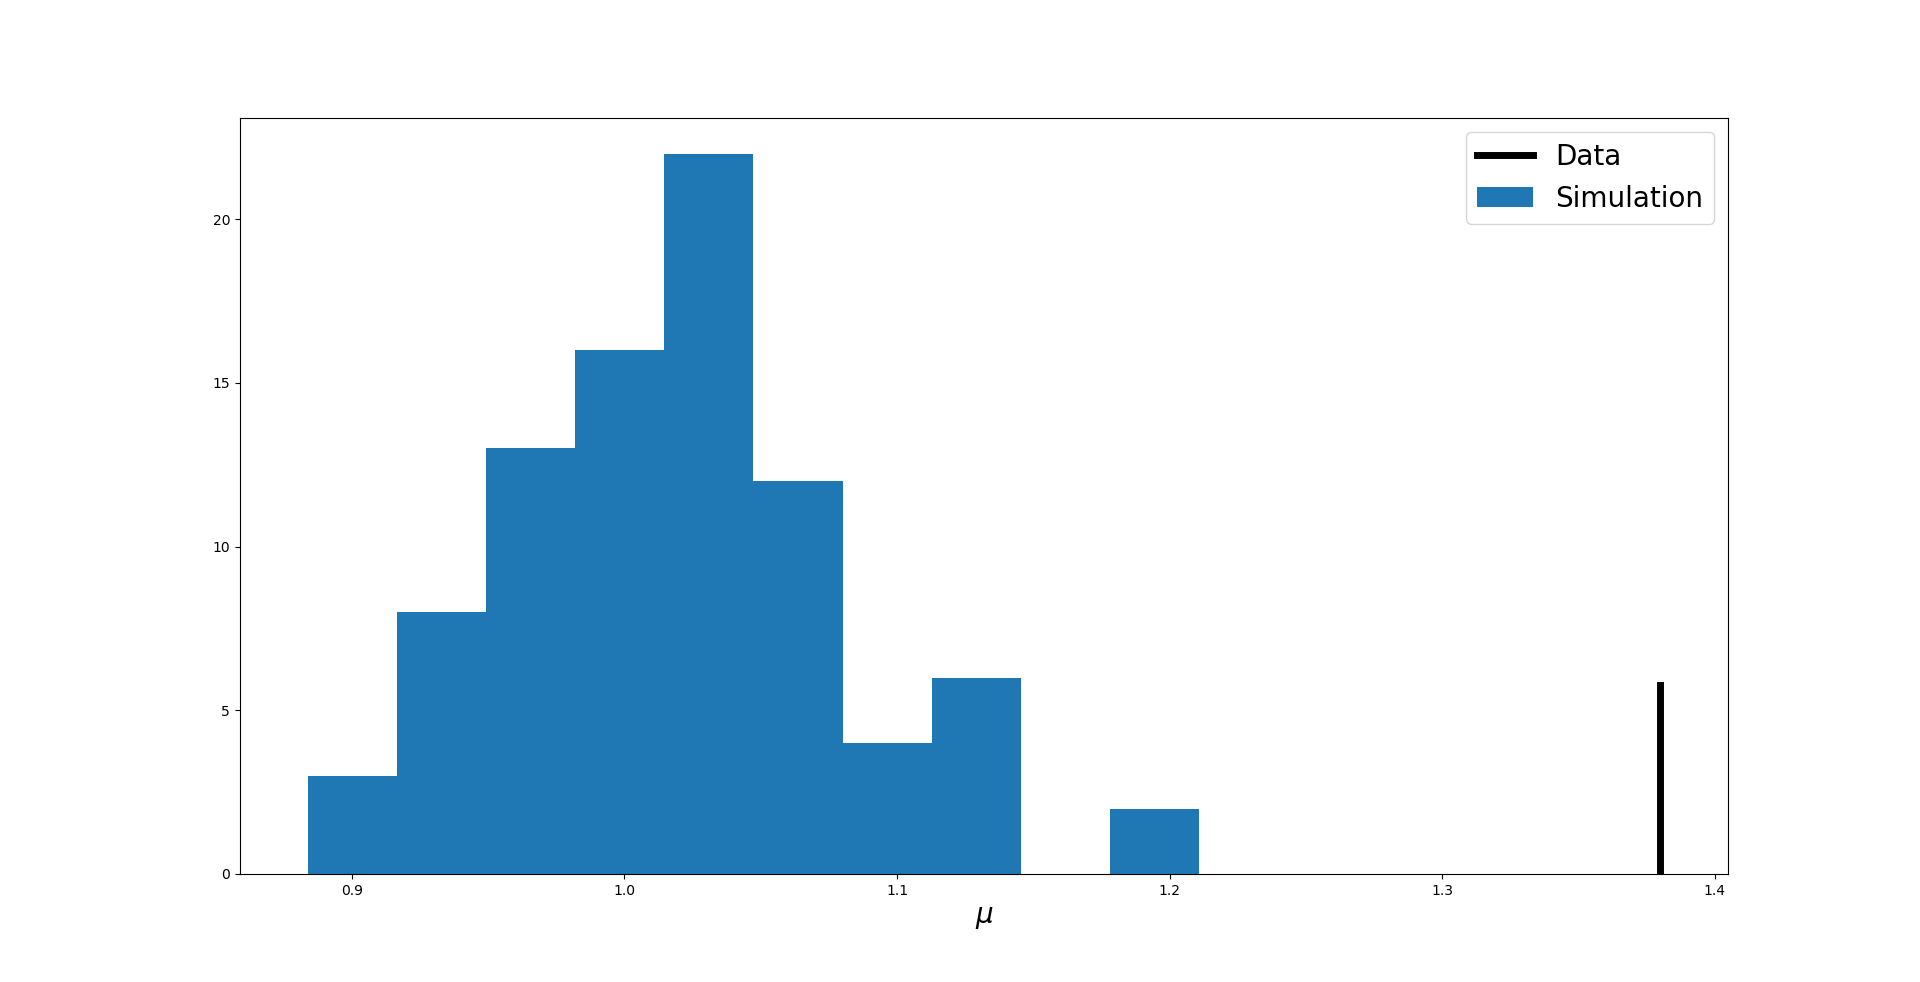
\includegraphics[width=\linewidth]{sag.png}
\end{figure}
\end{frame}

\begin{frame}{Detector sensitivity}
\begin{itemize}
\item For each value of $R_0, \zeta$ generate large number of datasets drawn from model-1.
\item Compute in which fraction ($\rho$) of datasets there is a detection over model-0.
\item Put $R_0, \zeta$ in  the $\rho$'th CL band.
\end{itemize}
\end{frame}

\begin{frame}{Upgrades before next run}
\begin{figure}[h]
  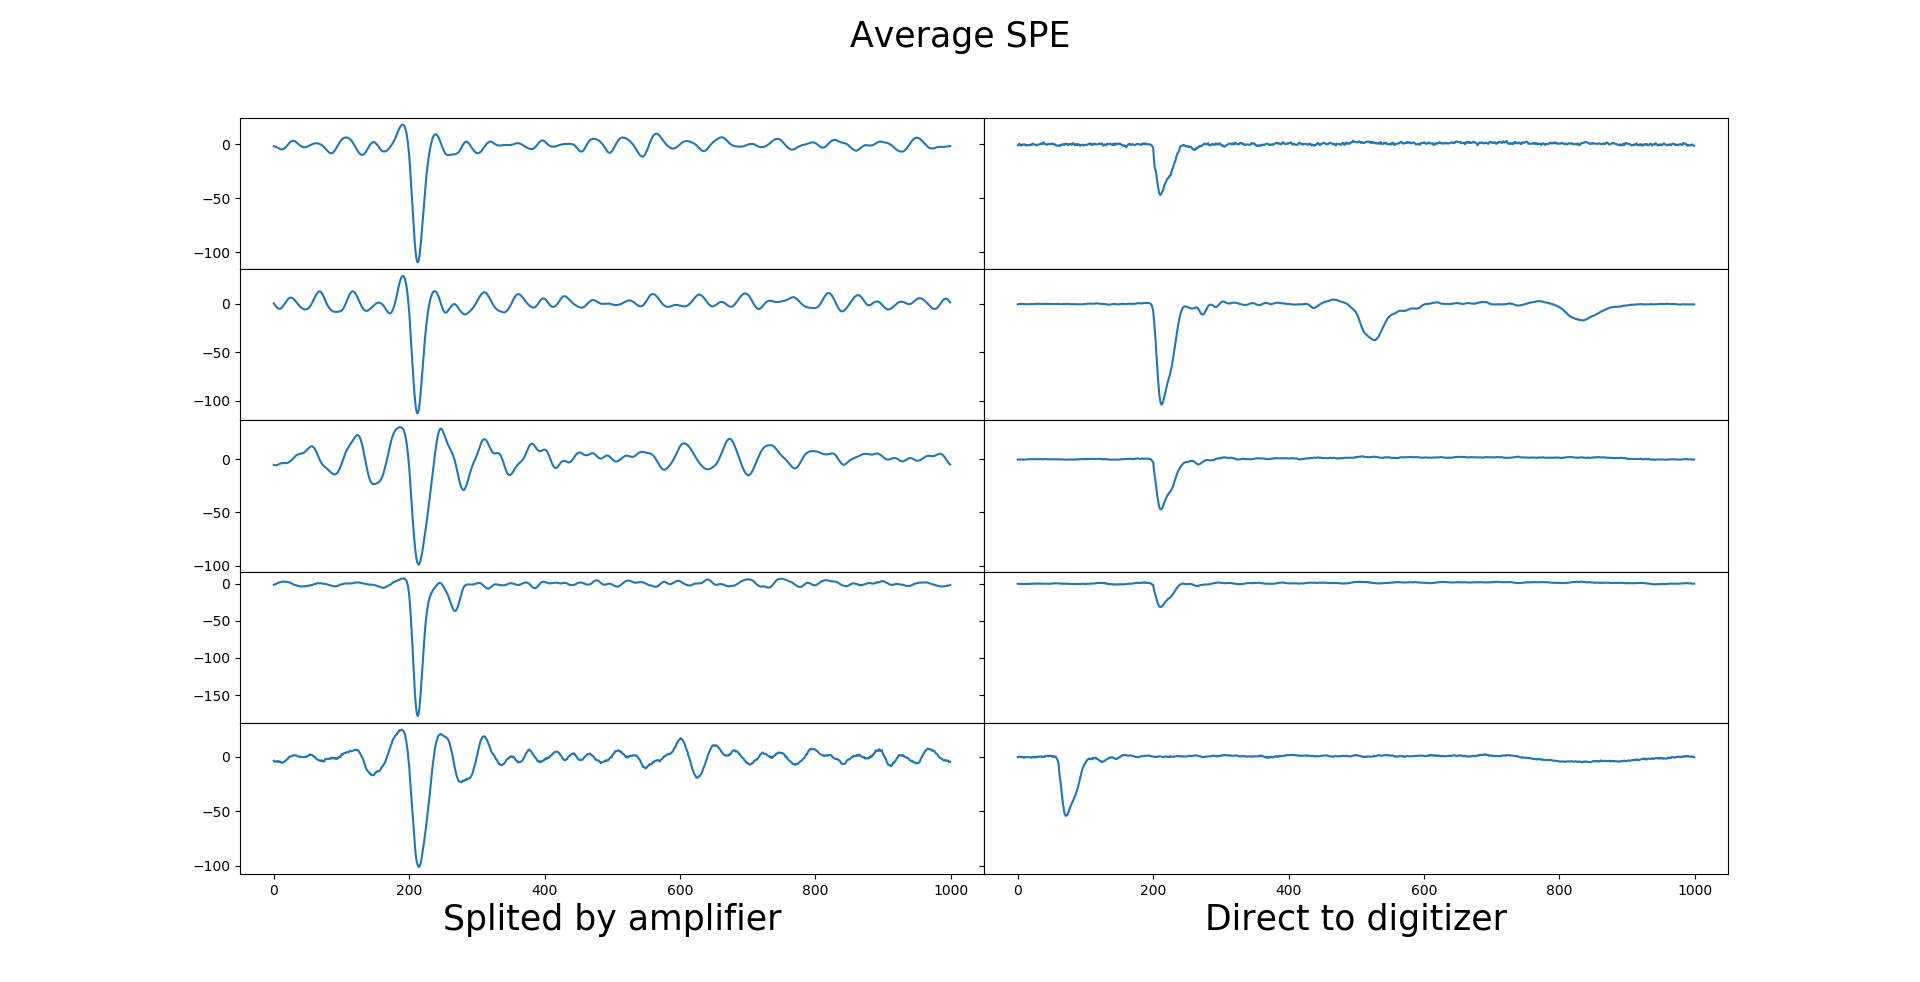
\includegraphics[width=\linewidth]{SPEs.png}
\end{figure}
\end{frame}

\end{document}


